\subsection{Introduction}
This reference manual describes the syntax and semantics of the
Feynstein programming language. The document is divided into
sections that aim to define the language conventions and
applications. For an introductory guide to working with Feynstein,
including sample programs, please refer to the Feynstein Language
Tutorial.

\subsubsection{Motivation}

Physics-based computer simulation is becoming increasingly popular as
a standard paradigm for scientific experimentation. For example,
physical simulation has revolutionized safety analysis of airplanes
and automobiles designs, testing of the effects of stress and strain
in the development of new materials, and our ability to further
understand molecular dynamics. Physical simulation allows for the
visualization of complex testing scenarios that are expensive,
dangerous, or merely impossible to recreate as in the case of testing
spacecraft and planetary rover designs. This ability to simulate
otherworldly scenarios with tangible physical accuracy has further
application to the film and gaming industries. With such myriad
application in the sciences and the arts, physical simulation demands
a flexible and intuitive configuration framework, one that is
accessible to researchers and artists with little programming
experience. 

The Feynstein programming language aims to provide such a framework by
offering the building blocks of physical simulation as highly
abstracted language types. Historically, if users wanted to have the
power of a full physical simulation engine, they had to either
purchase and learn very complex and expensive 3D simulation software,
which is costly and inflexible. For more specialized simulations,
users must extend a canned physics engine or implement their own,
traditionally in C++, which is not only time-consuming and
error-prone, but also requires programming expertise. For these
reasons, students of physics will learn simulation using a software
package like Matlab or Mathematica. These tools have the benefit of
abstracting much of the complexity of the task, but with the loss of
complexity comes a loss of control. Feynstein attempts to be a
midpoint between these two extremes. It is a language that allows for
the visual fidelity of a complex simulation package, but with the
ease-of-use that comes with a tool like Matlab.

\subsubsection{Extensibility}
Feynstein is fully object oriented and extensible, allowing for
straightforward customization of native forces and geometric
primitives. Users can additionally customize integration and rendering
methods, giving them full control of how their animation is calculated
and displayed.  Feynstein source files compile to Java executables,
and like Java, Feynstein supports extension of built-in types to
complex class hierarchies. Feynstein is thus not merely a language for
standard simulation, but also a platform upon which new simulation
algorithms may be developed.  As new geometric configurations, forces,
integration methods and collision detection methods are developed
using Feynstein, the language can continue to build upon itself. Our
ultimate goal is to offer a language in which any simulation can be
configured with as few tokens as would be required to simply describe
the scene in words.


\subsection{Top-Level Elements}

\subsubsection{Feynstein File Sections}
 
A Feynstein source program is comprised of three mandatory sections --
shapes, forces and properties -- and one optional section -- onFrame.
 
\paragraph{Shapes}
\label{sec:shapes}
The shapes section is where the geometry of the scene is
declared. This is essentially the modeling portion of the
code. Geometric primitives are instantiated here and assigned a unique
string identifier that can be reference latter when declaring forces
in the forces section. Below is an example of a shapes block for a
pendulum modeled as an edge and sphere.

\begin{verbatim}
shapes {
  shape Sphere(name="sphere1", radius=20cm, 
    location=(0cm, -40cm, 0cm));
  shape Edge (name="edge1", length=100cm, 
    location=(0cm, 60cm, 0cm), connects=("sphere1", null));
}
\end{verbatim}
 
\paragraph{Forces}

The forces section is where physical forces are assigned to the shapes
in the scene by name. The force section is where the animation is
defined. Different forces have unique configuration parameters, but
all non-global forces have an actsOn field that must be assigned to a
list of unique shape names already declared in the scene. Global
forces such as gravity of damping act on all objects in the scene. For
non-global forces, the number of names in this list must equal the
size of the forces' stencil. Below is an example of a spring force
acting upon the ball and string declared in \ref{sec:shapes} as
gravity pulls on the sphere.

\begin{verbatim}
forces {
  force SpringForce(actsOn="sphere1", length=40cm, strength=4);
  force GravityForce(gx=0, gy=0, gz=9.81N);
}
\end{verbatim}
 
\paragraph{Properties}

The properties section is the place to define all other aspects of the
simulation. Most notably, time integration and rendering methods are
declared here. Unlike the force and shapes sections, the properties
section has a default configuration if left empty. The default time
integration method is semi-implicit Euler and the default rendering
method is on-screen display. User defined properties that change the
appearance of the simulation -- such as textures and lighting -- find a
place in this section. An example of a simulation using verlet
time integration and video output (i.e. offline rendering) is shown
below.

\begin{verbatim}
properties {
  property VelocityVerlet(stepSize = 10ms);
  property FileOutput(name = "myScene.mov");
}
\end{verbatim}
 
\subsubsection{Frame Update Methods}
The frame update method (defined in the \texttt{onframe} block) of the
program allows the user to define any additional actions to be taken
every time a new frame is rendered in the simulation. This section is
largely user-defined and can be left empty. It is a block that is
executed every time the scene is stepped forward in time, but before
it is rendered. This gives the programmer an opportunity to observe or
change some of the properties of the objects in the scene before the
next frame is generated.

\subsubsection{Code Sample}

\begin{verbatim}
MyScene {
   /* This is where scene properties can be defined.
    * Anything that effects the entire scene goes here. */
   
   shapes {
     shape Sphere(name="sphere1", radius=20cm, location=(10,20);
     shape Cylinder(name="cylinder1", location=(0,0), 
       height=30cm, radius=10cm);
   }
   
   forces {
     force SpringForce(actsOn="cylinder1", attachesAt=(0,0), 
       pullsTowards=(-10, -10), strength=4N);
   }
   
   properties {
     property SemiImplicitEuler(stepSize=10tms);
     property VideoOutput();
     property FileOutput("myScene.avi");
     property AssertStability(margin=4);
   }

   onFrame {
     System.out.println("Rendered frame.");
   }
 }
\end{verbatim}

\subsection{Lexical Conventions}
 
\subsubsection{Statements}
As in Java, logical statements are separated with semicolons.
 
\subsubsection{Whitespace}
Lexical definition:

\begin{verbatim}
whitespace ::= " " | "\t" | "\n";
\end{verbatim}

Whitespace, as defined as spaces, tabs, and new lines, is solely used
to separate tokens.
 
\subsubsection{Comments}
Lexical definition:

\begin{verbatim}
comment ::= ( "//" (Letter | digit | operator | whitespace)* "\n" ) 
          | ("/*" (letter | digit | operator | whitespace)* "*/")
\end{verbatim}

Like Java, Feynstein supports single-line comments delineated with two
forward slashes "//". Feynstein supports multi-line comments
delineated at the beginning by a forward slash follwed by a star, "/*"
and at the end by a start followed by a forward slash, "*/".
 
\subsubsection{Identifiers and Keywords}

Identifiers are described by the following lexical definitions:

\begin{verbatim}
identifier ::= letter characters
characters ::= characters character | epsilon
character ::= letter | digit | '\_'
letter ::= lowercase | uppercase
lowercase ::= "a"..."z"
uppercase ::= "A"..."Z"
digit ::= "0"..."9"
\end{verbatim}

Identifiers are sequences of one or more alphanumerical characters and
underscores, and must begin with an alphabetical (ASCII Latin letter)
character.  Identifiers with the same spelling as a Java or Feynstein
keyword, boolean or null literal will not be recognized by the
compiler.

\paragraph{Primitive Types}
All of Feynstein's primitive types function like Java primitives in
that they are pre-defined, can be used as return values for functions,
and in that the value of a primitive-typed variable can only be
changed by assignment.  Feynstein has three special primitives, named
using Feynstein keywords \texttt{shape}, \texttt{force}, and \texttt{property}, and
corresponding to code blocks \texttt{shapes}, \texttt{forces}, and \texttt{properties},
respectively.  However, instead of assigning value and declaring
variables of these types using literals as in Java's or Feynstein's
other primitive types, Feynstein's special primitives are assigned to
either built-in or user-defined structures that require certain
specifications in order to be instantiated.  Feynstein's primitive
types also include the boolean, string, and int types found in Java.
They are assigned and operated on in the same way as the corresponding
Java types.  The number types, ints and decimals, are both declared
using literals as described in Section \ref{sec:numliterals}.

int decimal string boolean void shape force property

\paragraph{Section Declaration}

At some point within the code block constituting the scene to be
simulated and rendered, a \texttt{shapes}, \texttt{forces}, and \texttt{properties} block
must be declared.  These are declared by simply using the keyword
followed by a code block, which must contain declarations of any
shape, force, and property that is an element of the surrounding
scene.  In addition, the rendering method must be specified within the
properties code block.  The optional onFrame section is declared in
the same way.

\begin{verbatim}
codeSection ::= sectionName { codeBlock }
sectionName ::= shapes | forces | properties | onframe
\end{verbatim}

\subparagraph{Properties}

As mentioned above, there is more than one aspect of the scene that
must be declared in the properties code block.  There are property
primitives, which specify more technical aspects of the scene, such as
integration method and collision detectors.  These are declared in the
same way as the other two special primitives: with the key word
followed by the specific form the primitive is taking (i.e. Cylinder,
SemiImplicitEuler), and the parameters required to instantiate it.

The possible properties are EndTime, AssertStability, CameraView,
StabilityAssertTolerance, BoundingVolumeHierarchy, ProximityDetector,
VideoOutput and FileOutput.

\paragraph{Other Keywords}

The keywords \texttt{new} and \texttt{return} are used with Feynstein
classes and functions in the same way they are used in Java.  That is,
\texttt{new} is used to call the constructor to return a newly
instantiated object of the specified type, and \texttt{return} is used
within a function to escape the function block and specify the value
of the function call.

\subsubsection{Builder Syntax}
Feynstein adds a new way to construct objects, called "Builder
Syntax", which lets you use key-value pairs to call a series of
mutator methods. For example, to create a sphere with the name
sphere1, a radius of 20 centimeters, and centered at the origin, the
user can call \texttt{Sphere(name="sphere1", radius=20cm, location=(0, 0,
0));}. Builder syntax translates to a series of mutator calls in the
back end, meaning that it's super easy to write an API that works with
builder syntax. The earlier example translates to 

\begin{verbatim}
(new Sphere()).setName("sphere1").setRadius(20).setLocation(0, 0, 0)
\end{verbatim}

Note that the parentheses in the location parameter were flattened;
this means that it is easy to create parameters that can be set to a
tuple, such as location or color. Note, however, that these should be
treated as tuples and not lists of arbitrary length; for a property to
be set to a number of values, there has to be a method that takes
exactly that number of values. If you want a property to be set to
lists of arbitrary length, you will have to take an array as an
argument, and the end user of your API will not be able to use the
syntax described above.

\subsubsection{Literals}
 
\paragraph{Number literals}
\label{sec:numliterals}
All number literals are parsed as double precision floating point
literals, referenced as the decimal primitive type. Floating point
literals are described by the following lexical definitions:

\begin{verbatim}
decimal ::= pointfloat |exponentfloat
pointfloat ::= [intpart] fraction | intpart "."
exponentfloat ::= (intpart | pointfloat) exponent
intpart ::= int+
fraction ::= "." int+
exponent ::= ("e"| "E") ["+"|"‐"] int+
\end{verbatim}

Our implementation of the number literal is based on the hardware's
implementation of the Java double. Hence, range and overflow details
are left to the individual machines Java implementation. Note that for
simplicity of use, Feynstein supports only integer and decimal
(i.e. Java doubles).
 
\paragraph{Boolean literals}
Booleans are primitive types that evaluate to either one or zero. A
boolean in Feynstein is represented by a single bit in Java with the
following grammar:

\begin{verbatim}
boolean ::= true | false
\end{verbatim}

\paragraph{String literals}

Strings are sequences of characters. There is no character type in
Feynstein as we anticipate Strings only to be used for labels in
rendering and output messages. Individual characters are considered
strings of length one and represent at least 8 bits. String literals
can be enclosed in matching double quotes (") or single quotes (').
As of now, Feynstein supports strings consisting of ASCII characters
only. Unicode characters are not yet supported. String literals are
described by the following lexical definitions:

\begin{verbatim}
string ::= string stringchar | epsilon
stringchar ::= <any source character except "\"> | escapeseq
escapeseq ::= "\" character
\end{verbatim}

\paragraph{Time literals}
 
Time literals describe a unit of time. Time objects are implemented as
numbers in milliseconds and are described by the following lexical
definitions:

\begin{verbatim}
time ::= day
day ::= decimal "td" hour | hour
hour ::= decimal "th" minute | minute
minute ::= decimal "tm" second | second
second ::= decimal "ts" millisecond | millisecond 
millisecond ::= decimal "tms" | epsilon
\end{verbatim}

\paragraph{Spatial literals}
 
Spatial literals describe a unit of measurement. Spatial literals
represent a one-dimensional measure of length. Spatial literals can be
defined for higher dimensions using multiplication and exponent
operators. For example, 10m denotes 10 meters and
10m\textasciicircum{}2 and 10m*m denote 10 square meters. Furthermore,
spatial literals can be used in conjunction with time literals to
define velocities, accelerations, etc. For example, 10m/ts denotes 10
meters per second. Spatial literals are implemented in meters and are
described by the following lexical definitions:

\begin{verbatim}
length ::= meter | feet
meter ::= decimal "m" centimeter | centimeter
centimeter ::= decimal "cm" millimeter | millimeter
millimeter ::= decimal "mm" | epsilon
feet ::= decimal "ft" inch | inch
inch ::= decimal "in" | epsilon
\end{verbatim}

\paragraph{Mass literals}

Mass literals describe units of measure of the mass of objects. Mass
literals are implemented in kilograms and are described by the
following lexical definitions:

\begin{verbatim}
mass ::= kilogram
kilogram ::= decimal "kg" gram | gram
gram ::= decimal "g" milligram | milligram
milligram ::= decimal "mg" | epsilon
\end{verbatim}

\paragraph{Force literals}

All forces are measured in Newtons (N).

\begin{verbatim}
force ::= decimal "N" | epsilon
\end{verbatim}

\subsubsection{Delimiters}
The following tokens are designated as grammar delimiters:

\begin{verbatim}
+=    -=    /=        	
*=    =     (
)     {     }
/*    */    "
'     \
\end{verbatim}

\subsection{Expressions}

\subsubsection{Arithmetic Operations}
The following tokens are designated as arithmetic operators:
\begin{verbatim}
+ - / * \% \textasciicircum
\end{verbatim}

These operators retain their conventional operations; all are binary
operators, and the minus sign also functions as a unary negation
operator.

\subsubsection{Comparison Operations}

The following tokens are designated as arithmetic operators:
\begin{verbatim}
==    >=    <=   
<     >     !=
\end{verbatim}

These operators retain their conventional operations and all return a
boolean value. Comparison operators take a lower precedence than
arithmetic operations.

\subsubsection{Boolean Operations}

The following tokens are designated as boolean operators:
\begin{verbatim}
and    &&    or    ||    !
\end{verbatim}

Note that \texttt{and} and \texttt{\&\&} are synonymous, as are
\texttt{or} and \texttt{||}. These operators take a lower precedence
than both arithmetic and comparison operators. Boolean operations are
performed on the principle of lazy evaluation: for the expression
\texttt{a and b}, \texttt{b} is not operated if \texttt{a} is false,
and for the expression \texttt{a or b}, \texttt{b} is not evaluated if
\texttt{a} is true.

\subsection{Language model}

\subsubsection{Subsection types}
Like Java, Feynstein supports extension of object-oriented language
types. In the Feynstein language model, the notion of an object
``class'' is broken down into three types corresponding to the source
code subsections: shape, force, and property. Each type has properties
that must be defined by any new type definitions.

\subsubsection{Shapes}
The shape type represents a piece of geometry in the simulation
scene. Every shape has an underlying triangle mesh that defines its
geometry. An anonymous object of type shape can be instantiated
without definition given an input Object file (.obj). When a new shape
is instantiated, its underlying mesh is added to the global list of
triangles and a global list of vertices in the scene. These lists can
be indexed into by forces in the scene.

\paragraph{Shape accessors}
When defined in the shapes block, shapes are not assigned to a
variable. Rather, they are created anonymously, using the
\texttt{shape} keyword, and the compiler adds the shape to the
scene. Feynstein provides a mechanism for accessing these shapes after
they are created in the \texttt{\#} operator. The \texttt{\#} operator
takes the identifier after it, looks it up in the shapes table, and
returns it as a result; this allows for constructs like the following:

\begin{verbatim}
shapes {
  shape Sphere(name="sph1", radius=10m);
  System.out.println(#sph1.getRadius());
}
\end{verbatim}

\paragraph{Transformation operators}
Shapes can be scaled, translated, and rotated given a designated
operator and either a scalar or vector argument. Scalar arguments will
apply the transformations equally along all three axes. Vector inputs
are represented as (dx, dy, dz). Table \ref{tab:transform} shows the
operators and their corresponding definitions.

\begin{table}[h]\centering
  \begin{tabular}{r|l}
    Operator & Transformation \\ \hline
    \texttt{*} & Scale \\
    \texttt{->} & translate \\
    \texttt{\%} & rotate \\
  \end{tabular}
  \caption{Transformation operators}
  \label{tab:transform}
\end{table}

\paragraph{Predefined shapes}
The Feynstein language package includes pre-defined, re-sizable
shapes. The automatic discretzation of geometric primitives makes
Feynstein an excellent tool for building scenes without a separate
modeling tool to generate an Object file.  Built in shapes include:
\texttt{Sphere}, \texttt{Cylinder}, \texttt{Plane},
\texttt{RectangularPrism}, and \texttt{Tetrahedron}. The shapes and
the corresponding parameters are shown in Table \ref{tab:shapes}.

\begin{table}\centering
  \begin{tabular}{r|l}
    Shape & Parameters \\ \hline
    RectangularPrism & height, width, location, mass, name \\
    Cylinder & height, radius1, radius2 (optional), location, mass, name \\
    Sphere & radius, location, mass, name \\
    Tetrahedron & edges, location, mass, name \\
    Plane & normal, location, mass, name \\
    CustomObj & file, location, mass, name \\
  \end{tabular} 
\caption{Built-in shapes and their supported parameters}
\label{tab:shapes}
\end{table}

\paragraph{Custom shapes}
Custom shapes must be created in external 3D editing software and
exported as a Wavefront OBJ file. This can then be imported into
Feynstein using the \texttt{CustomObj} shape, which takes a \texttt{file} as a
parameter. Note that all textures defined in the OBJ file will be
ignored.

\subsubsection{Forces}
Force objects act on shapes in the scene to influence their
motion. All forces have an underlying force stencil. The force stencil
is a list of indexes into the global vertex list. Each force has an
optional fixed stencil size, the number of vertexes upon which it
acts. Although some forces may have special constructors for entire
shapes or a set of triangles, all forces can be defined with a unique
list of vertex indices equal in length to the stencil size. If the
stencil size is undefined, then the force is global and acts on all
vertexes in the scene.

\paragraph{Predefined forces}
\subparagraph{GravityForce}

A global gravitational force acting on each particle in the
simulation. Has three configurable components $(gx, gy, gz)$ which
express the vector acceleration due to gravity.

\subparagraph{DampingForce}

A global mass-based damping force acting to oppose the velocity of
each particle. The DampingForce has one parameter, $\gamma$, the
coefficient of the damping force acting on each particle. For a
particle with mass m and velocity $v = (vx, vy, vz)$, the damping force
is given by $f = -\gamma mv$.

\subparagraph{SpringForce}

A constraint force between two particles. The energy associated to the
spring force is $(\frac{k}{2L}) (||\vec{x}||−L)^2$, where $\vec{x} =
\vec{x}_j −\vec{x}_i$ is the vector between the two particles, $k$ is
the spring stiffness, and $L$ is its rest-length. The spatial
arrangement of this force can be seen in Figure \ref{fig:springf}.

\begin{figure}
  \centering
  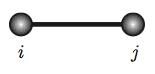
\includegraphics{figures/SpringForce}
  \caption{The spatial arrangement of particles for a \texttt{SpringForce}}
  \label{fig:springf}
\end{figure}

\subparagraph{RodBendingForce}

A RodBendingForce is a constraint force acting open three particles
that come to form a single hinge. The energy associated to the
rod-bending force depends upon the current angle $\theta$, as well as
some user-defined parameters: the undeformed lenghts of the edges
$\vec{ij}$ and $\vec{jk}$, the undeformed-angle $\bar{\theta}$, and
the force stiffness. The spatial arrangement of this force can be seen
in Figure \ref{fig:rodf}.

\begin{figure}
  \centering
  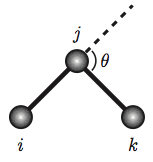
\includegraphics{figures/RodBending}
  \caption{The spatial arrangement of particles for a \texttt{RodBendingForce}}
  \label{fig:rodf}
\end{figure}

\subparagraph{ConstantStrainTriangleForce}

The ConstantStrainTriangleForce is based on a triangle stencil
involving three particles. This force resists both stretching and
compressing the triangular formation and depends upon the undeformed
lengths of the triangle edges, as well as the forces tensile modulus,
a measure of material stiffness, and its Poisson ratio, which relates
material compression to extraction. The spatial arrangement of this
force can be seen in Figure \ref{fig:trianglef}.

\begin{figure}
  \centering
  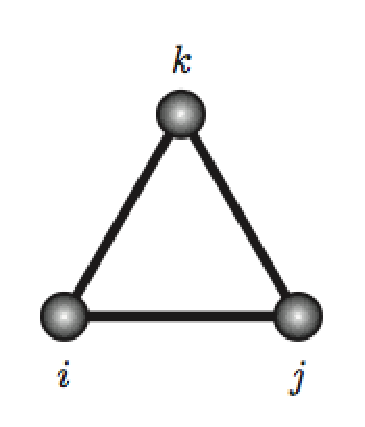
\includegraphics{figures/Triangle}
  \caption{The spatial arrangement of particles for a \texttt{ConstantStrainTriangleForce}}
  \label{fig:trianglef}
\end{figure}

\subparagraph{SurfaceBendingForce}

A SurfaceBendingForce is a constraint force that resists the bending
of a four-particle surface along its diagonal. The force energy is
based on the dihedral angle, $\phi$, which is the signed angle between
the normals of the two triangles in the configuration. The
SurfaceBendingForce class is thus parameterized by the undeformed
dihedralangle, the undeformed triangle edge lengths and the force
stiffness constant. The spatial arrangement of this force can be seen
in Figure \ref{fig:surfacef}.

\begin{figure}
  \centering
  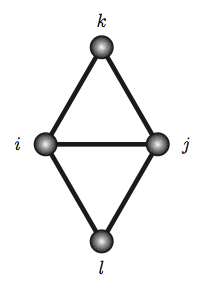
\includegraphics{figures/SurfaceBending}
  \caption{The spatial arrangement of particles for a \texttt{SurfaceBendingForce}}
  \label{fig:surfacef}
\end{figure}

\subsubsection{Properties}
Properties objects foremost include the non-optional properties of
simulation: time integration and rendering. Every simulation requires
a time-stepping method that defines force integration with each
update; and every simulation requires a method of outputting the
rendered scene. The property type can additionally be used to define
simulation features such as collision detection and response
frameworks, textures, lighting, and camera controls.

\paragraph{Predefined time integrators}

Feynstein provides two methods of integration, velocity Verlet and
semi-implicit Euler, for calculating changes to the scene over each
time step. Both the Verlet and semi-implicit Euler methods yield
more stable approximations of an object's trajectory than the explicit
Euler method, the other conventional method of calculation, which we
have omitted in the interest of accuracy. The integrators are defined
as \texttt{VelocityVerlet} and \texttt{SemiImplicitEuler} objects, and both require
only one parameter, the size of the time step to use in the time
integration calculations. This parameter should consist of a numerical
value and a time literal specifying the value's units.

\begin{verbatim}
properties {
  /* (other property declarations) */
  property SemiImplicitEuler(stepSize = 5ms);
}
\end{verbatim}

\paragraph{Predefined renderers}

Feynstein supports both online and offline methods of video output.
Online rendering means that when a Feynstein program runs, it displays
output directly on the screen. Online rendering produces an
interactive video output that lets the user use the mouse to change
the location of the camera, pan, tilt, and zoom during the
simulation. By default, Feynstein uses online rendering.  The use of
online rendering does not need to be explicitly specified.  If online
rendering is not wanted, how Feynstein should render the video needs
to be specified.  Offline rendering outputs a video file to a
specified file.

\begin{verbatim}
properties {
  property FileOutput(file="myScene.avi");
  property CameraView(location=(5m, 0, 0), 
    lookingAt=(0, 0, 0), fieldOfView=50);
}
\end{verbatim}

The user specifies where Feynstein should render the video using
the \texttt{FileOutput} property. The parameter of \texttt{File\-Output} is a
string specifying the file. Using offline rendering requires that the
camera position is specified using the \texttt{CameraView} property.

\paragraph{Predefined collision handlers}
Efficient collision detection and effective collision response are
essential to achieving accurate simulation for most scenarios. The
Feynstein language has built in property types for easy collision
detection and response.

\subparagraph{Detectors}

Feynstein supports a traditional, two-phase collision detection
framework. The narrow phase of detection supports both a basic proximity-based
method for classifying collisions, and more costly continuous-time detection for greater accuracy in
collision handling. To add a collision detection to your simulation, declare a
new \texttt{ProximityDetector} or \texttt{ContinuousTimeDetector} to the properties subsection. 

\begin{verbatim}                                                                                                                                             
properties {                                                                                                                                                 
  /*other property declarations...*/                                                                                                                         
  property ProximityDetector(proximity=1e-3);                                                                                                                
}                                                                                                                                                            
\end{verbatim}

\begin{description}
\item[ProximityDetector] A \texttt{ProximityDetector} requires one
  parameter: the minimum proximity that can be exhibited between two
  triangles before they are detected as colliding. At each simulation
  update, the \texttt{ProximityDetector} determines if any two
  triangles are going to violate this minimum proximity, and if so,
  marks them as colliding.

\item[ContinuousTimeDetector] A \texttt{ContinuousTimeDetector}
  requires no parameters and detects collisions at each simulation
  update by using each triangles current positions and velocities to
  determine at what time they would collide. If this collision time
  falls in between the current time and next update time, the two are
  marked as colliding.

  The optional broad phase of detection uses a spatial hierarchy, with
  support for a variety of bounding volumes, to determine pairs of
  triangles that are close enough to exhibit a collision. These
  potentially colliding triangles are then passed to the narrow phase
  detection, which would otherwise operate on the entire global
  mesh. This data structure is provided as an optimization to
  proximity-based collision detection and will automatically wrap all
  triangles in the global simulation mesh.

  To add broad phase detection to your simulation, declare a new
  \texttt{Bounding\-Volume\-Hierarchy} in the properties subsection of
  the Feynstein program. A \texttt{Bounding\-Volume\-Hierarchy}
  requires a bounding volume type specification: \texttt{AABB} for
  Axis-Aligned Bounding Boxes (default), \texttt{SPHERE} for Spheres,
  and \texttt{KDOP\_n} for n-degree K-Discrete Oriented Polytopes with
  $n \in {6, 14, 18, 26}$. Note that declaration of an broad phase
  detection property without a narrow phase detection property will
  cause a compiler error;

\begin{verbatim}
properties {
  /*other property declarations...*/
  property BoundingVolumeHierarchy(
    type=BoundingVolumeHierarchy.AABB, margin=1e-3);
  property ProximityDetector(proximity=1e-3);
}
\end{verbatim}
\end{description}

\subparagraph{Responders}

Collision response is handled by an additional property. Feynstein
includes two methods for responding to collisions. The first method, \texttt{SpringPenaltyResponder},  is a penalty-based method that uses a \texttt{SpringForce} between objects to resist their impact. The second method, \texttt{ImpulseResponder}, applies iterative impulses to object's velocities until collisions converge. All collision responders take a detector instance as a parameter. This detector will feed the responder it's collision set.

\begin{verbatim}
 properties { 
	/* other property declarations... */
        property BoundingVolumeHierarchy(margin=0.1);
        property ProximityDetector(proximity=0.1);
        property SpringPenaltyResponder(detector=0, stiffness=1000, proximity=0.1);
   }
\end{verbatim}
\begin{description}
\item[SpringPenaltyResponder] The \texttt{SpringPenaltyResponder}
  takes two parameters in addition to it's detector index: Thie spring
  stiffness used to resist collisions and the minumum proximity
  allowed between two triangles (i.e. the rest length of the
  spring). \texttt{SpringPenaltyResponder} takes a set of collisions
  from it's detector, which are flagged one of two canonical collision
  types: \texttt{VERTEX\_FACE} (one vertex and a three-vertex face)
  and \texttt{EDGE\_EDGE} (two two-vertex edges).

  The two points of the standard \texttt{SpringForce} stencil are then
  computed using the barycentric coordinates of the contact points
  within a face or along an edge. In a sense, the
  \texttt{SpringPenaltyResponder} holds a sub-\texttt{SpringForce} for
  each exhibited collision vertex set.

\item[ImpulseResponder] An \texttt{ImpulseResponder} takes one
  parameter in addition to it's detector index: The maximum number of
  iterations to perform when modifying object velocities until
  collisions converge. At each iteration, the
  \texttt{ImpulseResponder} projects the simulation state forward in
  time by updating object velocities and asking its detector to check
  for collisions. If any are found, impulses (either elastic or
  inelastic) are applied to object velocities, and the future
  simulation state is recomputed with the new velocities. This
  iterative step is performed until all collisions disappear or some
  maximum number or interactions is reached.
\end{description}

\paragraph{Camera Location and Orientation}

The CameraView property defines how the scene will appear to the
viewer. The location of the camera is given by a location (x, y, z) in
the scene. The camera has a default field of view of 45º, but this can
be changed when the camera is defined. By default, the camera is
located at the midpoint of the xy-projection of the objects in the
scene, and the default z value is calculated so that the camera can
see all objects in the scene.

\begin{verbatim}
properties {
  /*other property declarations */
  property CameraView(location=(0, 0, 3m), 
    lookingAt=(0, 0, 0), fieldOfView=30);
}
\end{verbatim}

\subsection{Execution Model}

\subsubsection{Code Blocks}
Code blocks consist of multiple statements executed as a group, and
the blocks can be nested. Code blocks are used to determine the
grouping of statements such as those that are part of a main Feynstein
code subsection or those that are part of a loop. The beginning of a code
block is delineated with a \texttt{\{}. The end of a code block is delineated
with a \texttt{\}}. Variables declared inside of a code block exist only
within that block of code.

\subsubsection{Stability Analyzers}

Stability analyzers are activated at run-time and throw exceptions
when the difference between the average kinetic energy at the
beginning of the simulation and the average kinetic energy at the
point in time being analyzed is not within the default tolerance
(1e-3), or a tolerance specified using the AssertStability property in
the properties block.

\begin{verbatim}
properties {
  /*other property declarations */
  property AssertStability(maxError=1e-6);
}
\end{verbatim}

\subsection{Grammar}

Note that, in the grammar below, the string \texttt{epsilon} is taken
to mean $\epsilon$, or the empty string.

\subsubsection{Tokens}

\begin{verbatim}
ID ::= (letter|'_')(letter | digit | '_')*
NUMBER ::= decimal
STRING ::= '(letter)*'

literal ::= timeLiteral | spatialLiteral 
            | massLiteral | forceLiteral
timeLiteral ::= day
day ::= decimal 'td' hour | hour
hour ::= decimal 'th' minute | minute
minute ::= decimal 'tm' second | second
second ::= decimal 'ts' millisecond | millisecond 
millisecond ::= decimal 'tms' | epsilon

spatialLiteral ::= meter | feet
	meter ::= decimal 'm' centimeter | centimeter
centimeter ::= decimal 'cm' millimeter | millimeter
millimeter ::= decimal 'mm' | epsilon
feet ::= decimal 'ft' inch | inch
inch ::= decimal 'in' | epsilon

velocityLiteral ::= spatialLiteral '/' timeLiteral | episolon

massLiteral ::= kilogram
kilogram ::= decimal 'kg' gram | gram
gram ::= decimal 'g' milligram | milligram
milligram ::= decimal 'mg' | epsilon

forceLiteral ::= decimal 'N' | epsilon

letter ::= lowercase | uppercase
lowercase ::= 'a'...'z'
uppercase ::= 'A'...'Z'
digit ::= '0'...'9'
decimal ::= pointfloat |exponentfloat
pointfloat ::= [intpart] fraction | intpart '.'
exponentfloat ::= (intpart | pointfloat) exponent
intpart ::= int+
fraction ::= '.' int+
exponent ::= ('e'| 'E') ['+'|'‐'] int+
\end{verbatim}

\subsubsection{File Structure and Expressions}

\begin{verbatim}
FeynsteinFile ::= ID { optCode shapeBlock optCode forceBlock 
  optCode propertyBlock optCode onframeBlock }
optCode ::= optcode statement | epsilon

shapeBlock ::= 'shapes' '{' shapes '}'
shapes ::= shapes shape ';' | epsilon
shape ::= 'shape' 'Sphere' '(' sphereParams ')' 
  | 'shape' 'Cylinder' '(' cylParams ')' 
  | 'shape' 'Plane' '(' planeParams ')' 
  | 'shape' 'RectangularPrism' '(' rectParams ')' 
  | 'shape' 'Tetrahedron' '(' tetParams ') 
  | 'shape' 'Cube' '(' cubeParams ')'
  | 'shape' 'FluidPlane' '(' fPlaneParams ')'
  | 'shape' 'ParticleSet' '(' pSetParams ')'
  | 'shape' 'ClothPiece' '(' pSetParams ')'
  | 'shape' 'RegularPolygon' '(' regPolyParams ')'
  | 'shape' 'SinglePointMass' '(' pointMassParams ')'
  | 'shape' 'SpringChain' '(' pSetParams ')'
  | 'shape' 'TriangleShape' '(' triangleParams ')'
  | 'shape' ID '(' userParams ')' 

sphereParams ::= sphereParams 'name=' STRING 
  | sphereParams 'radius=' NUMBER spatialLiteral 
  | sphereParams 'accuracy=' NUMBER
  | sphereParams 'location=(' NUMBER ',' NUMBER ')' | epsilon

cylParams ::= cylParams 'name=' STRING 
  | cylParams 'radius=' NUMBER spatialLiteral 
  | cylParams 'radius1=' NUMBER spatialLiteral ','  cylParams 'radius2=' NUMBER spatialLiteral 
  | cylParams 'height=' NUMBER spatialLiteral 
  | cylParams 'accuracy=' NUMBER
  | cylParams 'location=(' NUMBER ',' NUMBER ')' | epsilon

planeParams ::= planeParams 'name=' STRING 
  | planeParams 'normal '=' point | epsilon

tetParams ::= 'point1' '=' point ',' 'point2' '=' point ',' 'point3' '=' point ',' 'point4' '=' point ','

cubeParams ::= cubeParams 'sides' '=' '(' NUMBER spatialLiteral ',' NUMBER spatialLiteral ',' NUMBER spatialLiteral ')'
  | cubeParams 'allSides' '=' NUMBER spatialLiteral
  | epsilon 

fPlaneParams ::= fPlaneParams 'lengthX' '=' NUMBER spatialLiteral
  | fPlaneParams 'lengthY' '=' NUMBER spatialLiteral
  | fPlaneParams 'length' '=' NUMBER spatialLiteral
  | fPlaneParams 'subdivisions' '=' NUMBER | epsilon

pSetParams ::= pSetParams 'vert' '=' point 
  | pSetParams 'fixed' '=' NUMBER 
  | pSetParams 'velocity' '=' '(' NUMBER velocityLiteral ',' NUMBER velocityLiteral ',' NUMBER velocityLiteral ',' NUMBER velocityLiteral ')'
  | epsilon

regPolyParams ::= regPolyParams 'vertices' '=' NUMBER
  | regPolyParams 'radius' '=' NUMBER spatialLiteral | epsilon

pointMassParams ::= 'pos' '=' NUMBER | epsilon

userParams ::= userParams STRING '=' STRING 
  | userParams STRING '=' NUMBER 
  | userParams STRING '=' NUMBER literal
  | epsilon

point ::= '(' NUMBER ',' NUMBER ',' NUMBER ')'

forceBlock ::= 'forces' '{' forces '}'
forces ::= forces force ';' | epsilon
force ::= 'force' 'GravityForce' '(' gravityParams ')' 
  | 'force' 'DampingForce '(' forceParams dampParams ')' 
  | 'force' 'SpringForce' '(' forceParams springParams ')' 
  | 'force' 'RodBendingForce '(' forceParams rodParams ')' 
  | 'force' 'ConstantStrainTriangleForce '(' forceParams triangleParams ')' 
  | 'force' 'SurfaceBendingForce' '(' forceParams surfaceParams ')' 

forceParams ::= 'actsOn' '=' '#' STRING

gravityParams ::= 'gx' '=' NUMBER
  | 'gy' '=' NUMBER
  | 'gz' '=' NUMBER
  | epsilon

dampParams ::= 'coefficient' '=' NUMBER

springParams ::= 'length' '=' NUMBER spatialLiteral ',' 'strength' '=' NUMBER

triangleParams ::= 'youngs' '=' NUMBER ',' 'poisson' '=' NUMBER ','

rodBendingParams ::= 'strength' '='  NUMBER ',' 'angle' '=' NUMBER

surfaceBendingParams ::= 'strength' '=' NUMBER

propertyBlock ::= 'properties' '{' properties '}'
properties ::= properties property ';' |  epsilon
property ::= 'property' 'renderTo' '(' renderParams ')' 
  | 'property' 'endTime' '(' endParams ')' 
  |  'property' 'assertStability' '(' assertParams ')' 
  | 'property' eulerMethod '(' eulerParams ')' 
  | 'property' 'CameraView' '(' cameraParams ')' 
  | 'property' 'ProximityDetector' '(' 'proximityParams' ')' 
  | 'property' 'ContinuousTimeDetector' '(' cTParams ')'
  | 'property' 'BoundingVolumeHierarchy' '(' 'bvhParams' ')'
  | 'property' 'SpringPenaltyResponder' '(' springPenaltyParams ')'
  | 'property' 'ImpulseResponder' '(' impulseParams ')'

renderParams ::= 'VideoOutput' | 'FileOutput' '(' STRING ')' | epsilon

endParams ::= 'endAt=' TIME | epsilon 

assertParams ::= epsilon | 'margin=' NUMBER 

eulerMethod ::= 'VelocityVerlet' | 'SemiImplicitEuler'
eulerParams ::= 'stepSize=' timeLiteral

cameraParams ::= 'location' '=' '(' NUMBER ',' NUMBER ',' NUMBER ')'
  ',' 'lookingAt' '=' '(' NUMBER ',' NUMBER ',' NUMBER ')' 
  ',' 'fieldOfView' '=' NUMBER

proximityParams ::= 'proximity' '=' 'NUMBER'

bvhParams ::= 'margin' '=' NUMBER | 'margin' '=' NUMBER ',' 'type' '=' 'BoundingVolumeHierarchy.' 'volumeType'
volumeType ::= 'AABB'
num = '6' | '14' | '18' | '26'

springPenaltyParams ::= 'proximity' '=' NUMBER ',' 'detector' '=' NUMBER
  | 'proximity' '=' NUMBER ',' 'detector' '=' NUMBER ',' 'stiffness' '=' NUMBER 

impulseParams ::= 'detector' '=' NUMBER

onFrame ::=  'onFrame ' '{' onFrameAxns '}' | epsilon
onFrameAxns ::= statements statement | epsilon

statements ::= expression statements | statement statements | epsilon
statement ::= ID '=' expression | ID '=' tok
tok = ID | NUMBER | shape | force | property | timeLiteral
	expression ::= arithOperation | compOperation | boolOperation

arithOperation ::= NUMBER binOp NUMBER | '-' NUMBER
binOp ::= '+' | '-' | '/' | '*' | '%' | '^'

compOperation ::= NUMBER compOp NUMBER | ID '==' ID
compOp ::= '==' | '!=' |'>=' | '<=' | '>' | '<'

boolOperation ::= boolean boolOp boolean
boolean ::= 'TRUE' | 'FALSE' | compOperation | boolOperation
boolOp ::= 'and' | 'or' | '!'

conditional ::= 'if (' boolean '){' statements '}' elseBlock 
  | 'while (' boolean ') {' statements '}' 
  | 'do {' statements '} while (' boolean ');' 
  | 'for (' forInit ';' forExpr '; forUpdate ') {' statements '}'

elseBlock ::= 'else if (' boolean ') {' statements '} elseBlock 
  | 'else {' statements '}' | epsilon

forInit ::= expression | varDeclaration | epsilon
forExpr ::= expression forExpr | expression | epsilon
forUpdate ::= expression forUpdate | epsilon

\end{verbatim}
